% !TeX root = ../main.tex
% Add the above to each chapter to make compiling the PDF easier in some editors.

\chapter{Type Inference}\label{chapter:ti}
The previous chapter discusses the encoding of the type system in Z3. In this chapter, we explain how we build upon this encoding to provide a complete implementation for the static type inference. There are two phases for the type inference: constraints collection and constraints solving. In the phase of constraints collection, we traverse the input program, and generate constraints from the program constructs according to the type system. In the phase of constraints solving, we give the collected constraints to the SMT solver. If these constraints are satisfiable, a model is given in which a type is assigned to each variable in the program. Otherwise, the SMT solver reports the reason for the unsatisfiability. We discuss the methodology for constraints collection and constraints solving in this chapter.

\section{Type Inference Design}
We present here the main components of our type inference tool.
\subsection{Abstract Syntax Tree (AST)}
The AST of a program is a data structure describing the structure of the source code, where each node in the tree represents a construct occurring in the program.

Figure \ref{fig:ast} shows a visualization for the AST of the Python program below.

\begin{lstlisting}
def f():
	return "Hello world!"
f()
\end{lstlisting}
\begin{figure}
	\begin{mdframed}
		\centering
		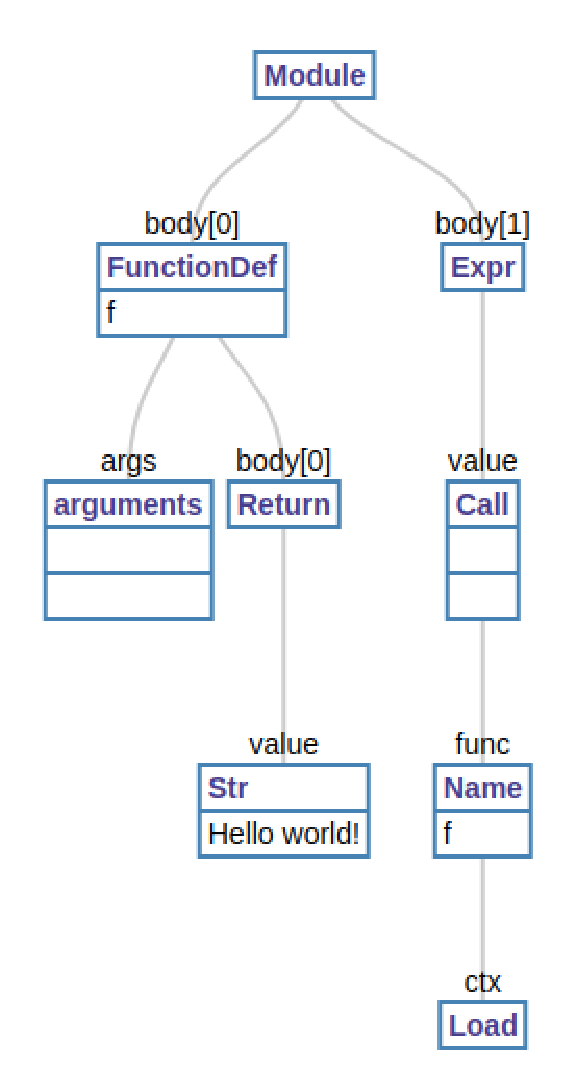
\includegraphics[width=50mm]{images/ast.eps}\\
	\end{mdframed}
	\caption{Abstract Syntax Tree (AST) for a Python program}
	\label{fig:ast}
\end{figure}

Our type inference works by traversing the AST in a depth-first manner, and gathering constraints defined by the type system along the way.
\subsection{Pre-analysis}\label{pre}
Before we attempt to infer the types of the input Python program, some pre-analysis is needed to configure the type inference.

The pre-analyzer takes the AST of the input program and provides the following information:

\begin{itemize}
	\item The maximum length of tuples that appear in the input program.
	\item The maximum number of function arguments that appear in the program.
	\item A mapping from all user-defined classes to their corresponding attributes and methods. It is important to differentiate between two kinds of these attributes: \textit{class-level attributes} and \textit{instance-level attributes}. Class-level attributes are those that are not specific to certain instances, and can be accessed with the class type itself, while instance-level attributes are those which are tied to the class instance during its instantiation or later on. For instance, the class \lstinline|A| in the following example has two attributes, namely \lstinline|x| and \lstinline|y|, where attribute \lstinline|x| is a class-level attribute while \lstinline|y| is an instance-level attribute.
	
	\begin{lstlisting}
class A:
	x = 1
	def __init__(self):
		self.y = 1
		
A.x  # valid
A().x  # valid
A().y  # valid
A.y  # invalid
	\end{lstlisting}
	
	Class-level attributes are detected by the pre-analyzer whenever it encounters an assignment statement in the top-level scope of the class in which the left-hand side is a normal variable.
	
	Instance-level attributes are recognized whenever they are assigned by accessing the first argument in the methods, like accessing \lstinline|self| argument in the above example. The inference can be pre-configured to only detect instance-level attributes that are defined within the \lstinline|__init__| method. This kind of configurations is explained in \ref{sub:config}
	
	Note that as far as the type inference is concerned, instance-level attributes also include class-level ones, that is every instance of a certain class can access any class-level attribute. However, instance-level attributes cannot be accessed by the class type itself.
	
	\item A mapping from all user-defined classes to their base classes or to \lstinline|object| if they do not explicitly inherit from other classes.
	\item The inheritance DAG which is used to generate the subtyping constraints discussed in the previous chapter.
\end{itemize}

In addition, the pre-analyzer does the following pre-processing to the user-defined classes:
\begin{itemize}
	\item Adds a default \lstinline|__init__| method to classes which neither contain nor inherit one.
	
	This default \lstinline|__init__| method has the following form:
	\begin{lstlisting}
def __init__(self):
	pass
	\end{lstlisting}
	Note that Python does not add this method for the classes which do not contain \lstinline|__init__|. However as what will be clear shortly, we add it to make the inference of the class instantiation easier.
	\item Propagates methods and attributes from base classes to their subclasses. The method resolution order which governs the order of this propagation is discussed later in this chapter.
\end{itemize}

\subsection{Context Hierarchy}
A context contains the information that a certain scope in the program holds. It contains a mapping from the variable names in this scope to the Z3 variables representing their types, which are evaluated to the correct types after solving the SMT problem. Every context also has references to its children contexts (which are created inside the scope of this context) and a reference to its parent context.

Below is a listing of the constructs which create new contexts:

\begin{itemize}
	\item \lstinline|if| statements.
	\item \lstinline|for| and \lstinline|while| loops.
	\item Function definitions
	\item Class definitions
	\item List, set and dictionary comprehensions
\end{itemize}

Figure \ref{fig:contexts} shows a tree representing the context hierarchy for the Python program below.

\begin{lstlisting}
x = [1, 2, 3]

class A:
	def f(self):
		pass
	def g(self):
		pass
	
for i in x:
	if True:
		pass
	else:
		pass
		
y = [i + 1 for i in x]
\end{lstlisting}

\begin{figure}[H]
	\begin{mdframed}
		\Tree[.{global} [.{A} {f} {g} ] [.{for} {if} {else} ] {list comp} ]
	\end{mdframed}
	\caption{Context hierarchy for a Python program}
	\label{fig:contexts}
\end{figure}


\subsection{Z3 Solver}
The Z3 solver is the main component in the type inference design. It is responsible for solving all the constraints imposed by the Python program semantics, or reporting that they are unsatisfiable.

We extend the solver class of the Z3 Python interface, such that during the instantiation of every solver instance, the following takes place:

\begin{itemize}
	\item The pre-analysis defined above in processed.
	\item The \textit{type sort} data-type is declared with all its constructors.
	\item The subtyping rules discussed in Chapter \ref{chapter:background} are initialized. 
\end{itemize}

At the end of the program inference, this solver is queried for a solution (model) to all the added constraints.

\subsection{Import Handler}
As the name suggests, the import handler is responsible for module importing during the type inference.

If the imported module is a built-in Python package, it retrieves the module from the corresponding stub file and stores the types of its contents in the appropriate context, otherwise, it reads the imported module from the disk and runs the inference algorithm to infer its types in a separate context, but within the same SMT problem.\\

Later in this chapter, we will discuss how different types of import statements are handled in our type inference.
\subsection{Stubs Handler}
As discussed earlier, \textbf{stubs} are files containing code which simulates other functionalities, like built-ins or low level code. A \textbf{stub function} is a function declaration which mocks some other function. The following function is a stub function which mocks the built-in function \lstinline|len|:

\begin{lstlisting}
def len(_: object) -> int:
	...
\end{lstlisting}

Stubs enable the type inference to infer the types of programs which use built-ins. The stubs handler is the module responsible for providing the types of the relevant stubs which are required by the program being inferred.

\subsection{Annotations Resolver}
PEP 3107 \cite{3107} introduced the ability to add function type annotations, while PEP 484 \cite{484} introduced the semantics of such annotations. The annotation resolver is responsible for translating a type annotation encountered in the program into the corresponding type-sort constructor.

For example, \lstinline|type_sort.list(type_sort.int)| is the translation of the type annotation \lstinline|List[int]|.\\

We will explain how these type annotations are useful in the type inference when we get to the inference of function definitions.
\subsection{Inference Configuration}\label{sub:config}
The user of the type inference has the ability to control the behavior of the type inference according to some pre-defined configurations. Each configuration is expected to have its gain and limitation. Some configurations, for instance, lead to a significant improvement in the inference performance, yet at the cost of rejecting a larger set of correct programs. We will discuss the current possible configurations when we get to the inference constraints related to these configurations.
\subsection{Hard Constraints vs. Soft Constraints}
An important addition to our type inference is introducing the ability to add soft constraints. \textbf{Hard constraints} are the constraints that \textbf{must} be satisfied by the program, such that if at least one hard constraint cannot be satisfied, the program is rejected by the type inference. On the other hand, \textbf{soft constraints} are those that can be violated, but the SMT solver tries to maximize the number of satisfied soft constraints. So a program violating some soft constraints is not rejected by the type inference. See the following example for illustration:

\begin{lstlisting}
def f(x):
	y = [1, 2, 3]
	return y[x]
\end{lstlisting}

Here, the list \lstinline|y| is indexed with variable \lstinline|x|. Therefore, the type of \lstinline|x| \textbf{must} be a subtype of \lstinline|int|, so a program in which the type of \lstinline|x| violates this constraint (e.g., having \lstinline|x| as a float) would be rejected. The constraint in this case is a hard one. Another hard constraint is added in the assignment statement \lstinline|y = [1, 2, 3]|, that the type of the array literal \lstinline|[1, 2, 3]| is a subtype of the type of variable \lstinline|y|. Moreover, a soft constraint is added that both the type of the list literal and the type of \lstinline|y| are the same. Without this soft constraint, the type of \lstinline|y| in the model given by Z3 might be \lstinline|object|, or any too general super type of the right-hand side (which is correct and sound, but not very accurate). So the purpose of the hard constraints is to provide a sound type inference, while that of the soft constraints is to increase its accuracy.
\section{Type Inference Rules}\label{sec:rules}
Having explained the main components of the type inference, we are now ready to discuss the constraints added for every construct in the Python program.
\subsection{Expressions Rules}
An \textit{expression} is any language construct that evaluates to a value. It can be a combination of one or more values, variables, operators and function calls. Every construct in Python that can be printed is an expression.

Below are some examples of Python expressions:
\begin{lstlisting}
1 + 2 / 3
-a
[1.2, 2.0, b]
[[1.1, 2.5], c]
{(i, i * 2) for j in d for i in j}
2 & 3
d[f]
(g, 2.0, a)
"string"
(1 is 2) + 1
i[o]
\end{lstlisting}

We present here the constraints that are generated by every expression in Python.

\subsubsection{List and Set Literals}
As discussed earlier, the elements of a single list or a set have to be homogeneous, that is all these elements have to be of the same type. So the \textit{elements type} of a list (or a set) literal is a super type of all the list (set) elements.

Assuming a function \lstinline|infer| which takes the AST node of the expression and returns a Z3 uninterpreted constant which represents its type, the inference of list literals is implemented as follows:

\begin{lstlisting}
def infer(node):
	...
	if isinstance(node, ast.List):
		elements = node.elts
		elements_type = new_z3_constant()
		
		for element in elements:
			current_type = infer(element)
			add_constraint(subtype(current_type, elements_type))
			
		return type_sort.list(elements_type)
	...
\end{lstlisting}

For example, the type of the list literal \lstinline|[1, 2.0, 3j]| can be \lstinline|List[complex]| or even \lstinline|List[object]|, since we assume \lstinline|complex| to be a super type of \lstinline|int| and \lstinline|float| and every type is a subtype of \lstinline|object|. With the soft constraint added, the type is restricted to \lstinline|List[complex]|.\\

The inference for sets is analogous to that of lists after replacing the list z3 constructor with the one for sets.


\subsubsection{Dictionary Literals}
Similarly to lists and sets, dictionaries should have homogeneous keys set and values set, and the type inferred for each of these sets is a super type of its elements. For example, the type inferred for the dictionary \lstinline|{1: "string", 2: 3.6}| is \lstinline|Dict[int, object]|, because \lstinline|object| is the common super type between \lstinline|str| and \lstinline|float|.


\subsubsection{Tuple Literals}
The type of a tuple includes information about the types of all its elements. So to get the type of a tuple, we first apply the expressions inference rules on all its elements. For example, the type of the tuple \lstinline|(1, "string", object())| is \lstinline|Tuple[int, str, object]|

\subsubsection{Binary Operations}
Binary operations combine two expressions, called operands, to produce a result expression. The type inference for binary operations in Python is not straightforward because the result type of every operation depends on different combinations of the types of the operands. We discuss here the constraints generated for every binary operation supported by Python.\\

\textbf{Addition (+)}:
The addition operation is either a numeric addition or a sequence concatenation. For the numeric addition, the type of the result is the super type of the types of the operands. This is encoded in Z3Py as follows:

\begin{lstlisting}
Or(
	And(subtype(left, complex), subtype(right, left), result == left),
	And(subtype(right, complex), subtype(left, right), result == right)
)
\end{lstlisting}

As for sequence concatenation, there are different cases to consider:

\begin{itemize}
	\item Lists concatenation: The result type is a list and the type of its elements is a super type of types of the elements in both operands.
	\item String (or byte string) concatenation: The two operands should be of the same type and so is the result.
	\item Tuple concatenation: The resulting type should be a tuple with the element types of both operands concatenated.
\end{itemize}

For brevity, we do not write the constraints for the sequence concatenation here.

Also, we do not currently consider operator overloading. However, this is not rejected by principle, these constraints can be extended to include classes which contain the method \lstinline|__add__|.

The listing below shows examples of different forms of the addition operation and their inferred types:

\begin{lstlisting}
1 + 1.0  # float
1j + 1.0  # complex
[1, 2, 3] + [4.0, 2]  # List[float]
"a" + "b"  # str
(1, "st") + (2.0, object())  # Tuple[int, str, float, object]
[1, 2, 3] + "a"  # Invalid
\end{lstlisting}

\textbf{Multiplication (*)}:
Multiplication in Python, again without considering operator overloading, is either numeric multiplication or sequence repetition.

Similarly to addition, the result type of numeric multiplication is the super type of the types of the operands. In case of sequence repetition, one of the operands must be a subtype of \lstinline|int| and the other one should be the sequence. In all the sequences except tuples, the result type is the same as the sequence being multiplied. Ideally in case of tuples, the result is a tuple type with the argument types of the operand tuple repeated by the operand number. However, resolving the exact numeric value is impossible statically. Therefore, we consider the result of tuple multiplication to a general Tuple type without specifying its elements. This is sound because as we will see shortly, any operation applied on this general tuple type (e.g., indexing) result in a sound general type like \lstinline|object|. \\
An important thing to notice in both addition and multiplication is that applying these operations on two \lstinline|bool| types results in an \lstinline|int| type. So this needs special handling during the constraints generation. For instance, the addition constraints are enhanced as follows:
\begin{lstlisting}
Implies(
	And(left == bool, right == bool),
	result == int
)

Implies(
	Not(And(left == bool, right == bool)),
	Or(
		# Addition constraints explained above
	)
)
\end{lstlisting}

\begin{lstlisting}
3 * 4.0  # float
[1, 2, 3] * 3  # List[int]
(1, 2) * 2  # Tuple[int, int]
True * False  # int
[1, 2] * 3.0  # invalid
\end{lstlisting}

\textbf{Division (/)}: Division is only applicable on numeric types. The result is \lstinline|complex| if at least one of the operands is of \lstinline|complex| type, otherwise it is a float. Note that this is different from floor division (//).

The constraints generated by a division operation are given below:

\begin{lstlisting}
And(
	types.subtype(left, complex), types.subtype(right, complex),
	Implies(Or(left == complex, right == complex), result == complex),
	Implies(Not(Or(left == complex, right == complex)), result == float)
)
\end{lstlisting}

\textbf{Other Arithmetic Operations (-, //, **, \%)}:
The remaining arithmetic operations (subtraction, floor division, exponentiation, modulo operator) exhibit similar behavior in terms of type inference. They can only be applied on numeric types and the result type is the super type of the types of the operands. \\

There is a single special case to consider in the modulo operator (\%). In addition to giving the division remainder, it can also be used in string formating. Therefore, a disjunction is added to the constraints in this case that the left operand is a \lstinline|str| type without restricting the right operand.

\begin{lstlisting}
"A string which contains a number %i}" % 1
\end{lstlisting}

\textbf{Bitwise Binary Operations (\&, \textrm{\^}, |, <<, >>)}:
Bitwise operations can only be applied on subtypes of \lstinline|int| types (\lstinline|int| and \lstinline|bool|). The result is \lstinline|int| in all cases except when we apply \&, \textrm{\^} or | on two \lstinline|bool| types, where in such case the result is \lstinline|bool|.

\subsubsection{Unary Operations}
Unary operations are applied on only one expression, called operand, and give a result expression. The supported unary operations in Python are unary \lstinline|-| (minus), unary \lstinline|+| (plus), unary \lstinline|~| invert, and \lstinline|not|.\\

For the plus and minus unary operations, the operand must be a subtype of \lstinline|complex|, and the result is \lstinline|int| if the type of the operand is \lstinline|bool|, otherwise it is the same type as the operand. As for the unary invert, the operand must be a subtype of \lstinline|int|, and the result is always of type \lstinline|int|.

The \lstinline|not| operation can by applied on any object and result in a \lstinline|bool| type.


\subsubsection{Boolean Operations}
There are two boolean operators in Python: \lstinline|and| and \lstinline|or|. Before explaining the inference for these operations, it is important to understand what a \textit{truth value} of an object is. In Python, every object can be tested for truth value, where each object can evaluate to \lstinline|True| or \lstinline|False| when used as test condition in \lstinline|if| or \lstinline|while| statements or in a boolean operation. The following values have a \lstinline|False| truth value:
\begin{itemize}
	\item \lstinline|None|
	\item \lstinline|False|
	\item Zero numeric values: 0, 0.0, 0j
	\item Empty collections: [], {}, ()
	\item Any object which has \lstinline|__len__| method which returns a zero or \lstinline|__bool__| method which returns \lstinline|False|.
\end{itemize}
Any other object has a \lstinline|True| truth value. \\

The result from \lstinline|and| operator is the first operand which has a \lstinline|False| truth value. If all the operands have \lstinline|True| values, then the result is the last operand. On the other hand, the result of \lstinline|or| operator is the first operand which has a \lstinline|True| truth value, or the last one if all have \lstinline|False| truth values.

\begin{lstlisting}
x = 1 and "str"
>>> x
"str"

x = 0 and "str"
>>> x
0

x = 1 or "str"
>>> x
1

x = 0 or "str"
>>> x
"str"
\end{lstlisting}

The constraints generated by a boolean operation are not simple to deduce since the result type depends on the values that the operands carry during runtime, and these values are impossible to be statically resolved. Specifically, the \lstinline|and| operator keeps evaluating the operands until an operand with a \lstinline|False| truth value is encountered. \lstinline|or| operator does the opposite. See the following example for illustration:
\begin{lstlisting}
a = function_which_returns_int()
b = function_which_returns_string()

x = a and b
y = a or b
\end{lstlisting}
If \lstinline|a| has a value zero at runtime, the type of \lstinline|x| will be the same as \lstinline|a|, \lstinline|int|, otherwise it will be \lstinline|str|. Conversely, \lstinline|y| will have type \lstinline|str| if \lstinline|a| has a zero value, otherwise it will have an \lstinline|int| type.

As mentioned, the values of \lstinline|a| and \lstinline|b| are impossible to be statically resolved. Therefore, the type of the result of a boolean operation is inferred to be the common super type between its operands. So the result of \lstinline|1 and 2.0| is \lstinline|float| and of \lstinline|1 and "str"| is \lstinline|object|.

\subsubsection{If (Conditional) Expression}
An if expression is an expression whose value depends on whether a certain condition is true or false.
\begin{lstlisting}
x = A if some_condition else B
\end{lstlisting}
This does the exact same thing as the following:
\begin{lstlisting}
if some_condition:
	x = A
else:
	x = B
\end{lstlisting}

The type of the value of the if expression is the common super type of the types of the true (A) and the false (B) values.

\subsubsection{Subscripts}
Subscript literals in Python end in square brackets containing some expression. For example, all the following are subscript literals:
\begin{lstlisting}
x[a]
x[a:b]
x[f()]
\end{lstlisting}

There are two kinds of subscripts in Python: \textit{indexed} subscript and \textit{sliced} subscript. A sliced subscript contains one or two colons \lstinline|:|, e.g., \lstinline|x[a:b]|. Any other subscript is an indexed subscript. \\

In Python, any type which contains the \lstinline|__getitem__| method can be indexed or sliced. However, for simplicity, here we only consider built-in types. We explain later in this chapter how we enhance the type inference to account for user-defined classes which implement the \lstinline|__getitem__| method. \\

In our type system, only strings (and byte strings), lists, dictionaries and tuples support \textbf{indexing}:

\begin{itemize}
	\item For strings, the index must be a subtype of \lstinline|int| and the result is a \lstinline|str|.
	\item For lists, the index is a subtype of \lstinline|int| and the result is the type of the list elements.
	\item For tuples, the index must be a subtype of \lstinline|int|, and the result is the common super type between all the tuple elements. This is because it is not possible to statically resolve the value of the index, so we cannot know which element the indexing is referring to. As for the general tuple type \lstinline|Tuple|, the result of indexing is constrained to be \lstinline|object|.
	\item For dictionaries, the index type should be the same as the inferred type of the dictionary keys, and the result type is the type of the dictionary values.
\end{itemize}

Disjunctions for all the above possibilities are added whenever an index subscript is encountered during the inference traversal. \\

As for \textbf{sliced} subscripts, only strings, lists and tuples support slicing. The slicing keys must be a subtype of \lstinline|int|. For all types except tuples, the result type from slicing is the same as the sliced object. For tuples, the result is the general tuple type \lstinline|Tuple| because resolving the slicing ends is impossible statically.

\subsubsection{Comprehensions}
Comprehensions are constructs which enable the programmer to create lists, sets or dictionaries in a natural and elegant way from any other iterable object. The following set comprehension creates a set \lstinline|x| which contains the square of all values in another iterable \lstinline|y|.

\begin{lstlisting}
x = {i * i for i in y}
\end{lstlisting}

This is equivalent to the following in a mathematical syntax:
\begin{lstlisting}[language=, mathescape, basicstyle=\sffamily]
x = {i * i | i $\in$ y}
\end{lstlisting}
The expression \lstinline|i in y| in the above example is called a \textit{generator expression} while the expression \lstinline|i * i| is called the comprehension element.

The inference for comprehensions works by creating a local context for the generator, and constraining the generator target (\lstinline|i| in the example above) in this local context according to the generator iterable (\lstinline|y|). Then by having the Z3 constant corresponding to type of the target in the local context, the type of the comprehension element can be inferred by generating the expressions constraints explained above.

For the example above, assuming the type of \lstinline|y| is constrained to be \lstinline|List[int]|, then the type of \lstinline|i| is inferred as \lstinline|int| in the local context of the generator expression. Then the type of the set elements is inferred from the multiplication inference rules explained above: \lstinline|int * int := int|. So the comprehension result will have a result of \lstinline|Set[int]|. Assuming that \lstinline|x| is the z3 constant representing the type of the iterable in the generator expression and \lstinline|y| represents the type of the generator target, the following axion is generated during the inference of the generator expression:
\begin{lstlisting}
And(
	subtype(x, iterable(y))
)
\end{lstlisting}
Now the local context of the comprehension is as follows:
\begin{lstlisting}
context = {
	'i' : y
}
\end{lstlisting}
Then the multiplication constraints are added on the type of the variable \lstinline|i|. \\

Note that, the generator expressions can be chained (nested). See the following example for illustration:

\begin{lstlisting}
x = [[1, 2, 3],
     [4, 5, 6],
     [7, 8, 9]]
	 
y = [i for j in x for i in j]
\end{lstlisting}

The list \lstinline|y| contains the list \lstinline|x| after flattening all its inner lists (\lstinline|[1, 2, 3, 4, 5, 6, 7, 8, 9]|). The inference for chained generators works by applying the inference rules on the generator targets in the order they appear in the comprehension. So after solving all the constraints, the type of \lstinline|j| in the above example is inferred to be \lstinline|List[int]| (because \lstinline|x| is \lstinline|List[List[int]]|), and the type of the second generator target \lstinline|i| (which is also the comprehension element) is inferred to be \lstinline|int|, and the type of y is then \lstinline|List[int]|.

In addition to generators chaining, the comprehension itself can be nested.
\begin{lstlisting}
x = [[1, 2, 3],
     [4, 5, 6],
     [7, 8, 9]]
	 
y = [[i * 2 for i in j] for j in x]	 
\end{lstlisting}
The variable \lstinline|y| is now a 2D array with the same dimensions as x, where each element in \lstinline|y| is the double of the corresponding one in \lstinline|x|.

The inference for comprehensions nesting works exactly the same as normal comprehensions: The comprehension \lstinline|[i * 2 for i in j]| is treated first, and \lstinline|j| is constrained to be \lstinline|List[int]|. Now having the the z3 constant representing type of \lstinline|j| in the local context of the comprehension, the type of the inner comprehension can be constrained with the same rule. Therefore after solving the SMT problem at the end, the inner comprehension will have the type \lstinline|List[int]| and the outer one will have the type \lstinline|List[List[int]]|, which is the type of \lstinline|y|.\\

The inference for dictionary comprehension works the same way as lists and sets. The only difference is that the comprehension element consists of a mapping instead of a single expression. The following example creates a dictionary comprehension which maps every value in a list to its square.
\begin{lstlisting}
{a: a * a for a in [1, 2, 3]}
\end{lstlisting}

After applying the inference rules on the generator expressions, the types for the dictionary keys and the values in the the comprehension element are inferred in the local context of the generators.

\subsubsection{Variables Inference}
The context contains a mapping from variable names to the Z3 constants that represent their types. The inference for variables is as simple as looking up the name of the variable in this mapping.

The variables are stored in the context with the assignment statements, function definitions or class definitions. The inference for these constructs are explained in the upcoming sections.

\subsection{Statements Axioms}
A statement is a complete instruction that can be executed by the Python interpreter and performs a certain action. Note that every expression written alone in a separate line of code is also a statement.

We explain here how the type inference works for different statements in our type system.

\subsubsection{Assignment Statements}
There are several variations of the assignment statement in Python. However there is one important common constraint that is generated for all the variations, that is the right-hand side of the assignment must be a subtype of the left-hand side. In other words, the assignment target in any assignment statement must be a super type of the assignment value.

\begin{lstlisting}
	target = value  # value <: target
\end{lstlisting}


\textbf{Simple Variable Assignment}: The simplest variation of the assignment is the variable assignment:
\begin{lstlisting}
	variable = value
\end{lstlisting}
If the target variable already exists in the context, the above subtyping constraint is imposed on the Z3 constant which this variable is mapped to in the context, otherwise, a new Z3 constant is created on which the subtyping constraint is applied. For illustration, assume that the context initially has the following mapping:
\begin{lstlisting}
{
	'x': x_z3_constant
}
\end{lstlisting}
Assume that these two assignment statements are encountered:
\begin{lstlisting}
	x = 1
	y = "string"
\end{lstlisting}
Since variable \lstinline|x| already exists in the context, no new Z3 constant is created for it, and the constraint is added on the Z3 constant it is mapped to, \lstinline|x_z3_constant|:
\begin{lstlisting}
	subtype(int, x_z3_constant)
\end{lstlisting}
As for the variable \lstinline|y| not being in the context, a new Z3 constant is created for it and inserted to the context. The context now has the following contents:
\begin{lstlisting}
{
	'x': x_z3_constant,
	'y': y_z3_constant
}
\end{lstlisting}
And the following constraint is also generated for the variable \lstinline|y|:
\begin{lstlisting}
	subtype(str, y_z3_constant)
\end{lstlisting}

\textbf{Tuple and List Assignment}
\begin{lstlisting}
x, y = 1, "str"
[a, b] = [1, 2]
\end{lstlisting}

The inference for this kind of assignment is similar to the variable assignment. The difference is that the target elements are checked one by one if they already exist in the context, and similarly, a new Z3 constant is created for the targets which do not exist in the context.

Since the lists in our type system have homogeneous elements, the types involved in the list assignment must also have the same type. So the assignment \lstinline|[a, b] = [1, "str"]| will lead both variables \lstinline|a| and \lstinline|b| to have type \lstinline|object| (the common super type of \lstinline|int| and \lstinline|str|).

\textbf{Subscript Assignment}
\begin{lstlisting}
a[x] = b
a[x:y:z] = b
\end{lstlisting}
Any class which implements \lstinline|__setitem__| method is capable of performing subscript assignment. However for simplicity and similarly to subscript expressions inference, we only consider built-in types here. We explain later how to extend the inference to include user-defined classes as well.

Strings, byte strings and tuples are immutable objects, so they do not support subscript assignment. So whenever a subscript assignment is encountered, a constraint is generated that the subscripted object is not \lstinline|str|, \lstinline|bytes| or any \lstinline|Tuple| type.\\

The last type of assignment statements is attribute assignment (e.g., \lstinline|a.x = b|). We will discuss this type of assignment after explaining the inference for class definitions and the attribute access for class instances.\\

It is worth noticing the role of the soft constraints in the assignment inference. The result of the subtype constraint added for every assignment statement may make the inference not very accurate. For example, the assignment \lstinline|x = 1| may lead \lstinline|x| to have type \lstinline|float| or even \lstinline|object|, since \lstinline|float| and \lstinline|object| are super types of \lstinline|int|. So a soft constraint is added that the type of \lstinline|x| is \lstinline|int|. See the following example:
\begin{lstlisting}
x = 1
x = 2.5
\end{lstlisting}

The above code generates two hard constraints and two soft ones. The hard ones state that the type of x is a super type of both \lstinline|int| and \lstinline|float|. The first soft constraint assigns the type \lstinline|int| to \lstinline|x| and the second one assigns the type \lstinline|float| to it. In the result model, only one soft constraint is satisfied (the second one), giving the type of \lstinline|x| to be \lstinline|float|, which satisfies the two hard constraints.

\subsubsection{Body (Block of Statements) Type}
A code block in Python is a group of Python statements starting with the same indentation tabs. We assume that every statement in Python has a \lstinline|None| type, except the \lstinline|return| statement which has the type of the value it returns. This makes it easier to infer the type of a block and also, as we will explain shortly, the return type of functions. The type of a code block is the common super type of all non-\lstinline|None| (non \lstinline|return|) statements, or \lstinline|None| if all the block statements have a type \lstinline|None|. See the following example for illustration:
\begin{lstlisting}
def f(x, y):
	z = x + y
	return z
	
def g(x, y):
	x[0] = y
\end{lstlisting}
In the function \lstinline|f|, the first statement sets the type of \lstinline|z| to be the result from the addition constraints explained before between \lstinline|x| and \lstinline|y|. This assignment statement itself has a \lstinline|None| type. The second statement has a type equal to the type value it returns: \lstinline|z|. The type of the body of the function \lstinline|f| is the super type of all the non-\lstinline|None| statements in the body, which is the type of \lstinline|z|. In the function \lstinline|g|, all the body statements have a \lstinline|None| type, so the type of the function body is \lstinline|None|.

\subsubsection{Control-Flow Statements}
A control-flow statement decides on two or more paths to follow during the program execution. The inference for these kind of statements is tricky because the way the types in the context are affected depends on which path was taken, which is not always possible to resolve statically. We present here what constraints are generated for the control-flow statements in Python, and how the context is affected by the paths choice. \\

There are three variants of control-flow statements in Python: \lstinline|if| statements, \lstinline|for| loops and \lstinline|while| loops. However, the constraints generated for these statements are the same, except that an additional constraint for the loop variable is generated in the case of \lstinline|for| loops. \\

Each control-flow statement has a required body block and an optional else block, and a separate local context is created for each. If one branch introduces a new variable, it will only be added to the parent context (which contains the control-flow statement) if the other branch also defines this variable. This prevents attempting to use a variable which might have not been defined. See the following example for illustration:

\begin{lstlisting}
if some_condition:
	x = 1  # This is the first time x is defined
	print(x)
else:
	pass
	
print(x) # Invalid: x might have not been defined.
\end{lstlisting}
In the above example, using the variable \lstinline|x| outside the local scope of the \lstinline|if| body block is not allowed, since the flow might have taken the \lstinline|else| path, where in this case variable \lstinline|x| would not exist. \\

The type of a control-flow statement is the common super type between its branches. For example, the type of the following \lstinline|if| statement is \lstinline|object|, which is the super type of both \lstinline|int| and \lstinline|str|.

\begin{lstlisting}
if some_condition:
	return 1
else:
	return "string"
\end{lstlisting}


\subsubsection{Deletion}
The dynamic nature of Python allows the programmer to delete a value at runtime. The type inference supports all kinds of deletion except attribute deletion. Attribute deletion is not supported because in a nominal static type system, all instances of a certain type are expected to have the same attribute everywhere in the program.

The simplest kind of deletion is normal \textbf{variable deletion}. The deleted variable is simply removed from the context. Also, when a variable is deleted in one branch of a control-flow statement, it is also deleted from the context, because determining which branch was taken is not possible statically, so it is safer to assume that it was deleted.

For example, using the variable \lstinline|x| after the following \lstinline|if| statement is unsafe, because the \lstinline|then| branch might have been taken, where the variable \lstinline|x| is deleted.
\begin{lstlisting}
x = 1
if some_condition:
	del x
else:
	pass
	
print(x)  # Invalid: x might have been deleted.
\end{lstlisting}

The second variant of deletion is \textbf{subscript deletion}. Every subscriptable object, with the exception of immutable objects, can be used in subscript deletion. So constraint is generated when a subscript deletion is encountered that the subscripted object is mutable.
\subsection{Function Definitions Inference}\label{func}
The inference for function definitions is the main motivation behind adopting SMT to the solve the type inference problem. For a program composed of only assignment statements, the type for every variable can be easily resolved by tracking the type of the value it is assigned to. However for function arguments, there is no origin for the type to track. The types of these arguments are solely based on how these arguments are used in the function body and how this function is called; hence the idea of constraints solving evolved.\\

As stated earlier, a local context for the function is created. Each argument in the function is mapped to a newly created Z3 constant in this local context, where this fresh constant is totally free from any constraints. Then the statements inference rules are applied on the body of the functions. These rules impose constraints on the types of the function arguments. The return type of the function is the constrained type of the body block of the function. If a function has no \lstinline|return| statement, then the return type is \lstinline|None|. At the end, Z3 will assign types to the constants corresponding to the types of the arguments which satisfy all the imposed constraints. Let us illustrate the functions inference with the following example:
\begin{lstlisting}
def f(x, y, z):
	a = x + y
	z += [1, 2]
	return z[a]	
\end{lstlisting}
Initially, we create the context which contains the Z3 constants representing the types of function arguments.

\begin{lstlisting}
context = {
	'x': x_z3_constant,
	'y': y_z3_constant,
	'z': z_z3_constant
}
\end{lstlisting}
The first statement \lstinline|a = x + y| generates the addition constraint, and the type of variable \lstinline|a| is stored in the context.
\begin{lstlisting}
context = {
	'x': x_z3_constant,
	'y': y_z3_constant,
	'z': z_z3_constant,
	'a': addition_result
}
\end{lstlisting}
The second statement \lstinline|z += [1, 2]| generates another addition constraint. According to the addition constraints explained before, lists can only be added to lists. Therefore, we type of \lstinline|z| is constrained to be \lstinline|List[T]| such that \lstinline|int <: T|. The last \lstinline|return| statement generates the subscript constraint. From the subscript rules, we know that lists can only be indexed with subtypes of \lstinline|int|. Putting this constraint together with the addition constraint on which the type of variable \lstinline|a| depends, we restrict the type of \lstinline|a| to be a subtype of \lstinline|int|, and so are the types of \lstinline|x| and \lstinline|y|. Therefore the type of the function \lstinline|f| is inferred to be, according to the syntax of PEP 484 \cite{484}, \lstinline|Callable[[A, B, List[T]], T]|, such that \lstinline|A <: int|, \lstinline|B <: int| and \lstinline|int <: T|. Z3 will pick only one model for \lstinline|A|, \lstinline|B| and \lstinline|T|. So, for instance, the types \lstinline|Callable[[int, int, List[int]], int]|, \lstinline|Callable[[bool, int, List[float]], float]| and \lstinline|Callable[[bool, bool, List[complex]], complex]| are all valid types for \lstinline|f|. Further constrains from function calls might narrow down these types and exclude some of them.\\

In order to increase the accuracy and to make the type inference more deterministic, we make use of soft constraints in all the contexts that give multiple possibilities because of the subtyping relationship. Specifically in this example, a soft constraint is added in the  addition operation that the type of the addition result is the same as the two operands. So with the soft constraints being added, Z3 will assign the type \lstinline|Callable[[int, int, List[int]], int]|. to \lstinline|f|.

\subsubsection{Arguments Default Values}
A function in Python can have zero or more default values for the function arguments. If these default values exist, they are used to constraint the initial types of the function arguments. The type of every argument which has a default value must be a super type of the type of this value. See the following example:

\begin{lstlisting}
def f(x, y=1):
	return x + y
\end{lstlisting}

From the default value of the argument \lstinline|y|, and assuming that \lstinline|T| denotes the Z3 constant representing the type of \lstinline|y| in the context, a new constraint is generated that \lstinline|int <: T|. Additionally, a soft constraint is added here that both \lstinline|T| and \lstinline|int| are the same. So the type of the function \lstinline|f| given by the Z3 model is \lstinline|Callable[[int, int], int]|.\\

In order to accommodate the default arguments in the function type encoding in Z3, a new attribute, which has \lstinline|Int| sort, is introduced in the function constructor of the \textit{type sort} data-type declaration. This attribute represents the number of default arguments this function has. Recalling the function constructor declaration from chapter \ref{chapter:ts}, the new accessor is added to the accessors array of the constructor.
\begin{lstlisting}
accessors = [("func_{}_defaults_args".format(cur_len), IntSort())]
\end{lstlisting}

\subsubsection{Function Type Annotations}
The programmer also has the ability to write type annotations for the function arguments as well as the return type. PEP 484 \cite{484} introduced the semantics for writing the type annotations. For example, a list of integers will have the type annotation \lstinline|List[int]|. By default, these type annotations are not type-checked. In our tool, these annotations are useful in reducing the number of generated constraints, and hence improving the performance of the type inference. When an argument is annotated in a function definition, the indicated type is used instead of creating a new uninterpreted Z3 constant.
\begin{lstlisting}
def f(x: int, y: int, z):
	...
\end{lstlisting}
The above function will have an initial local context with the following contents:
\begin{lstlisting}
context = {
	'x': int,
	'y': int,
	'z': z_z3_constant
}
\end{lstlisting}

\subsubsection{Parametric Polymorphism}
The dynamic structural typing of Python gives a polymorphic nature to its functions. Since all the types are evaluated at runtime and no types are attached to the function arguments or the returned value, a function can accept a value of any type for its arguments which allows the operations performed inside the function. See the following example for illustration:
\begin{lstlisting}
def add(x, y):
	return x + y
	
a = add(1, 2)  # type := int
b = add("a", "b")  # type := str
c = add([1, 2], [3, 4])  # type = List[int]
\end{lstlisting}
The function \lstinline|add| can accept different argument types, and the return type depends on which types are passed as the function arguments. One limitation of depending on SMT solving to infer the type of the function is that the solver picks only one model. So referring to the above example, the function \lstinline|add| can only perform either numeric addition or sequence concatenation, but not both. Thus, the approach described so far prevents this kind of polymorphism, and the above program will be rejected. To work around this limitation, we introduced the ability to annotate the function with a generic type variable. The syntax for these type variables follow the syntax introduced in PEP 484 \cite{484}.

Re-writing the above example with generic type variables:

\begin{lstlisting}
from typing import TypeVar, List

T = TypeVar("T")
U = TypeVar("U", [int, str, List[T]])

def add(x: U, y: U) -> U:
	return x + y
\end{lstlisting}
Now the function \lstinline|add| can accept any type which is indicated in the possibilities of the type variable \lstinline|U|, and it returns the type which is unified with this type variable during the function call. We will describe later in Section \ref{sec:call} how this unification algorithm works.

However, introducing generic type variables comes with its limitations. Functions containing generic type variables are handled separately from Z3. Accordingly, no Z3 constant is created for any function that contains a generic type variable, and any function that contains one must be fully type-annotated (i.e., there must be a type annotation for every argument and the return of the function). Another consequence of treating these functions separately from Z3, they cannot be used as a first class object, that is they cannot be passed as function arguments. The only supported way to use functions with generic type variables is via direct function calls.
\subsection{Class Definitions Inference}
Classes provide a way for creating new types in Python. Each instance of any class has a set of attributes attached to it, which identify its state, behavior and properties. We explain here how the type inference works for defining new classes. \\

\subsubsection{Pre-analysis}
As mentioned in Section \ref{pre}, the pre-analyzer provides the following information about class definitions prior to running the type inference algorithm:
\begin{itemize}
	\item A mapping from classes to methods: \lstinline|methods|
	\item A mapping from classes to instance-level data attributes: \lstinline|instance_level_attrs|
	\item A mapping from classes to class-level attributes: \lstinline|class_level_attrs|
	\item A mapping from classes to their base classes, or to \lstinline|object| if they do not have any: \lstinline|bases|
\end{itemize}
Then as described in Chapter \ref{chapter:ts}, all the user-defined classes are encoded in the \textit{type sort} data-type, and Z3 uninterpreted constants are created for every method and data attribute which will represent their corresponding types in the generated model, and each class is mapped to the Z3 constants representing its own attributes.

\subsubsection{Attributes and Methods Inference}
When a class definition statement is encountered, a local context is created for this class. Then the statements inside the class (its methods and attributes declarations) are also traversed depth-first starting from the class node itself. The type of each statement is then constrained according to the inference rules described for expressions, statements and functions. After the traversal of the class contents is done, the types added to the local context of the class are unified with the corresponding Z3 constants the class is mapped to, which represent the types of the attributes of this class. Let us discuss the following example for illustration:
\begin{lstlisting}
class A:
	x = 1
	def __init__(self):
		self.a = 1
	def get_a(self):
		return self.a
\end{lstlisting}
The pre-analyzer gives the following mappings:
\begin{lstlisting}
class_level_attrs = {
	'A': ['x', '__init__', 'get_a']
}
instance_level_attrs = {
	'A': ['x', 'a', '__init__', 'get_a']
}
methods = {
	'A': ['__init__', 'get_a']
}

bases = {
	'A': ['object']
}
\end{lstlisting}
And the mapping from the class to the Z3 constants is also created:

\begin{lstlisting}
z3_consts = {
	'A': {
		'x': attr_x_z3_const,
		'__init__': attr_init_z3_const,
		'get_a': attr_get_a_z3_const,
		'a': attr_a_z3_const
	}
}
\end{lstlisting}
It is worth mentioning that the first argument in any instance method (handling static methods is discussed shortly), called the method receiver, is always automatically constrained to have the type of class itself. So \lstinline|self| in the above examples will have the type \lstinline|A|. \\

At the beginning, the local context of the class is empty. Then the class contents is traversed and the constrains are generated as described before. After the statement \lstinline|x = 1| is encountered, attribute \lstinline|x| is constrained to be a super type of \lstinline|int|. In the function \lstinline|__init__|, we constraint the type of the instance-level data attribute \lstinline|self.a| to be a super type of \lstinline|int|. The types of the methods \lstinline|__init__| and \lstinline|get_a| are constrained as described in Section \ref{func}. In the end, the local context of the class \lstinline|A| looks as follows:
\begin{lstlisting}
context = {
	'x': x_z3_constant,
	'__init__': init_z3_constant,
	'get_a': get_a_z3_consant
}
\end{lstlisting}
Then at the end of the class inference, the following unification constraints are added to the SMT problem to define the types of the class attributes:

\begin{lstlisting}
context['x'] == z3_consts['A']['x']
context['__init__'] == z3_consts['A']['__init__']
context['get_a'] == z3_consts['A']['get_a']
\end{lstlisting}
Note that the type of the attribute \lstinline|self.a| is not included in this unification, since it is already unified by the attribute assignment statement in the \lstinline|__init__| method.

\subsubsection{Method Decorators}
Decorators provide a mechanism to dynamically alter the functionality of a function. Decorators in general are not supported in our type inference, since they may dynamically alter type-related functionalities of the functions. Currently, the only supported decorators are \lstinline|@staticmethod| and \lstinline|@abstractmethod|. \\

The inference for methods decorated with \lstinline|@staticmethod| works as instance methods, except that the first argument is not unified with the class instance. We also impose a restriction that static methods can only be invoked on class types; they cannot be called on class instances. The reason for such restriction is to provide more type flexibility and lift variance restrictions which are imposed on the inherited methods. The variance restrictions are to be discussed shortly. The inference of calling static methods will be explained when we get to method calls inference in Section \ref{sec:call}. \\

As for \lstinline|@abstractmethods|, the body type of the method is ignored, and any subclass is enforced to override any abstract method that appears in any of its super classes.

\subsubsection{Inheritance}
Every class definition can define zero or more classes to inherit from. Inheriting from a class explicitly defines a \textit{subtype} relationship between the subclass and the parent class. All the methods which exist in the super classes and are not explicitly implemented in the subclass are inherited.
\begin{lstlisting}
class A:
	def f(self):
		pass

class B(A):
	pass
	
B().f()
\end{lstlisting}

Class \lstinline|B| inherits from class \lstinline|A| and does not implement the method \lstinline|f|, so the method \lstinline|f| is inherited by \lstinline|B| from \lstinline|A|. However, things get more complicated in the presence of multiple inheritance. See the following example:

\begin{lstlisting}
class A:
	def f(self):
		return 1

class B:
	def f(self):
		return "str"
		
class C(A, B):
	pass
	
x = C().f()  # What is the value (and type) of `x`?
\end{lstlisting}

Now determining which \lstinline|f| function is being called is not trivial. This is where the method resolution order (MRO) becomes crucial. MRO is the order in which methods and attributes are resolved in the presence of multiple inheritance. Python 3 uses the \textit{C3 linearization} algorithm to determine the MRO. We briefly explain how this algorithm works.

\subsubsection{C3 Linearization}
The algorithm works by defining the linearization of every class. The linearization of a class is a function of the linearizations of its parent classes (if any). The linearization of a class is a list containing the class itself followed by a unique merge of the linearizations of the parents of this class and a list of these parents.

\begin{lstlisting}
linearization[A] = [A] + merge(parents_linearizations, parents)
\end{lstlisting}
The merge function is responsible of merging several lists into one list. It works as follows:
\begin{itemize}
	\item Select the first head of the lists which does not appear in the tail of any other list.
	\item Remove the selected item from all the lists where it appears as a head and add it to the output list.
	\item Repeat the above two steps until all the lists are empty
	\item If no head can be removed and the lists are not yet empty, then no consistent MRO is possible.
\end{itemize}
For example, merging the lists \lstinline|[B, A]| \lstinline|[C, A]|, \lstinline|[B, C]| will be as follows:
\begin{itemize}
	\item Select \lstinline|B| to be the good head and append it to the result list, since it does not appear in the tail of any list.
	\item Remove \lstinline|B| from all the lists. Now the lists are \lstinline|[A]|, \lstinline|[C, A]| and \lstinline|[C]|.
	\item Similarly, remove the head \lstinline|C|. Now the lists are \lstinline|[A]|, \lstinline|[A]| and \lstinline|A|.
	\item Select \lstinline|A|. Now all the lists are empty and the result of the merge is \lstinline|B, C, A|.
\end{itemize}
Let us see a more concrete example:
\begin{lstlisting}
class A:
	def f(self):
		return A

class B(A):
	pass

class C(A):
	def f(self):
		return C
		
class D(B, C):
	pass
	
x = D().f()
\end{lstlisting}
Method \lstinline|f| in class \lstinline|A| returns the type of the class \lstinline|A| itself. Similarly, the one in \lstinline|C| returns the type of class \lstinline|C|. Now which of these is inherited by class \lstinline|D|? Let us calculate the linearization of each class.
Let function \lstinline|L(x)| denote the linearization of class \lstinline|x|.
\begin{lstlisting}
L[A] = [A] + merge([object]) = [A, object]
L[B] = [B] + merge(L(A), [A])
     = [B] + merge([A, object], [A])
     = [B] + [A, object]
     = [B, A, object]
Similarly,
L[C] = [C, A, object]
L[D] = [D] + merge(L(B), L(C), [B, C])
     = [D] + merge([B, A, object], [C, A, object], [C, B])
     = [D] + [B, C, A, object]
     = [D, B, C, A, object]
\end{lstlisting}
Now to determine which method \lstinline|f| is inherited by class \lstinline|D|, we traverse the linearization of class \lstinline|D| and stop at the first class we encounter which implements the method \lstinline|f|. So class \lstinline|D| inherits method \lstinline|f| from class \lstinline|C|, because it is the first class in the linearization of \lstinline|D| which implements \lstinline|f|, and the type of the variable \lstinline|x| is inferred to be \lstinline|Type[C]|.

\subsubsection{Overridden Methods Variance}
Variance is a topic that usually comes with any nominal type system which defines subtype relationships between its types. There are four forms of variance: invariance, covariance, contra-variance and bi-variance. We will explain these forms in the context of functions. See the following classes structure for illustration:
\begin{lstlisting}
class A: ...
class B(A): ...
class C(B): ...
\end{lstlisting}

And the following function:
\begin{lstlisting}
def f(x: B): ...
\end{lstlisting}

Function \lstinline|f| accepts an argument \lstinline|x| of type \lstinline|B|.

\textbf{Invariant} functions whose arguments are restricted to a certain type do not accept neither super types nor subtypes of these types. So an invariant \lstinline|f| can only accept \lstinline|B| instances, not \lstinline|A| or \lstinline|C|.

\textbf{Bi-variant} functions accept both super types and subtypes. So a bi-variant \lstinline|f| will accept instances of \lstinline|A|, \lstinline|B| and \lstinline|C|.

\textbf{Covariant} functions accept subtypes but not super types. So a covariant \lstinline|f| accepts \lstinline|B| and \lstinline|C|, but not \lstinline|A|.

\textbf{Contra-variant} functions accept super types but not subtypes. A contra-variant \lstinline|f| accepts \lstinline|A| and \lstinline|B|, but not \lstinline|C|.

Let us add some methods to the classes above:

\begin{lstlisting}
class A:
	def f(self, x: int) -> int:
		return x
		
class B(A):
	def f(self, x):
		return x
\end{lstlisting}
Class \lstinline|A| has a method \lstinline|f| which accepts subtypes of \lstinline|int| as its argument and returns an \lstinline|int| type. Class \lstinline|B| inherits from \lstinline|A| and overrides the method \lstinline|f|. Assume a function \lstinline|foo| which accepts an instance of \lstinline|A| as its argument.

\begin{lstlisting}
def foo(a: A):
	x = a.f(1)
	# .. more statements which use `x` ..
\end{lstlisting}
Now \lstinline|x| is expected to have the type \lstinline|int| (the return type of method \lstinline|f| in class \lstinline|A|). Since \lstinline|B <: A|, then \lstinline|B| instances can be used whenever \lstinline|A| instances are expected. So, \lstinline|B| instances can be passed as the argument for \lstinline|foo|. Therefore, the return type of method \lstinline|f| in class \lstinline|B| \textbf{must} also allow all the operations that are executed in the body of the function \lstinline|foo|. So it must be a subtype of the return type of the overridden method \lstinline|f| in class \lstinline|A|. Therefore, the return type of overriding methods is covariant with the return type of the overridden methods.

On the other hand, any argument passed to the method \lstinline|f| in class \lstinline|A| must be also compatible with the corresponding argument in class \lstinline|B|. So the types of arguments in the overriding method in \lstinline|B| \textbf{must} be super types of the corresponding ones in the overridden method. Therefore, the types of arguments of the overriding methods are contra-variant with the corresponding ones in the overridden methods. \\

One thing to consider is the use of default arguments in the presence of these variance constraints. Referring back to the example, any call to method \lstinline|f| in class \lstinline|f| takes into account that it might be a call to the method \lstinline|f| in class \lstinline|B| instead. So any call to \lstinline|f| on an \lstinline|A| instance must also be valid as a call to \lstinline|f| on a \lstinline|B| instance. Therefore, the number of required arguments which have no default value in the overriding method in the subclass must be less than or equal to the one in the overridden method, and the total number of arguments in the overriding method in the subclass must be greater than or equal to the total number of arguments in the super class. For example, assume the following method exists in class \lstinline|A|:
\begin{lstlisting}
def g(self, x, y=1):
	pass
\end{lstlisting}
Then the calls \lstinline|a.g(1)| and \lstinline|a.g(1, 2)| are both valid, where \lstinline|a| is an instance of class \lstinline|A|. These two calls must also be valid if they were invoked on any instance of a subclass of \lstinline|A|. So if class \lstinline|B| overrides method \lstinline|g|, the maximum number of required arguments it can have is one, and the minimum number of total arguments it can have is two (ignoring the first \lstinline|self| receiver argument).\\

Formally, if the number of required arguments and arguments with default values in the super class are \lstinline|a| and \lstinline|b| respectively, and those of the subclass are \lstinline[mathescape]|a$'$| and \lstinline[mathescape]|b$'$|, then the following conditions must hold:
\begin{lstlisting}[mathescape]
a$'$ $\leq$ a 
a$'$ + b$'$ $\geq$ a + b
\end{lstlisting}

In the presence of multiple inheritance, if a method exists in more than one super class, then the overriding methods must satisfy the variance conditions described above with the methods in all the super classes, because an instance of a subclass can be used where an instance of any of the super classes is expected. For example, if a class \lstinline|D| extends both classes \lstinline|B| and \lstinline|C|, then an instance of \lstinline|D| can be used where an instance of \lstinline|B| or \lstinline|C| is expected.

\subsubsection{More on Multiple Inheritance}
Supporting multiple inheritance comes with a lot of scenarios to consider. One of them is the call to \lstinline|super()|. The function \lstinline|super| calls the next method in the method resolution order. So a \lstinline|super| call in a certain method can refer to many different methods, depending on from where this call is originating. See the following example:
\begin{lstlisting}
class A:
	def f(self): ...
		
class B(A):
	def f(self):
		return super().f()
	
class C(A):
	def f(self):
		return super().f()

class D(B, C):
	def f(self):
		return super().f()
\end{lstlisting}

If asked which class \lstinline|super| the method \lstinline|f| in class \lstinline|B| is referring to, the most intuitive answer is class \lstinline|A|. However, this is not always the case. The \lstinline|super| call might have originated from method \lstinline|f| in class \lstinline|D|, and as we just discussed, the \lstinline|super| call refers to the next method in the MRO. Class \lstinline|D| has the linearization \lstinline|[D, B, C, A]|. So the super in \lstinline|D| will refer to \lstinline|B|, and that in \lstinline|B| refers to \lstinline|C|. This makes the inference for the \lstinline|super| call very complicated, since the super-methods may have different number of arguments or may even not exist. Assume that the class \lstinline|C| did not have the function \lstinline|f|, then calling \lstinline|super| from \lstinline|f| in class \lstinline|B| would still be fine since it may refer to \lstinline|f| in class \lstinline|A|, and such resolution is not always possible to resolve statically. Adding support for the \lstinline|super| call is still under research.\\

Another tricky case that comes with multiple inheritance is to decide which data attributes are inherited by a subclass from the super classes. See the following example:

\begin{lstlisting}
class A:
	def __init__(self):
		self.x = None
class B:
	def __init__(self):
		self.y = None

class C(A, B):
	pass
\end{lstlisting}
Class \lstinline|C| inherits from both \lstinline|A| and \lstinline|B|, and according to the linearization of \lstinline|C|, only the \lstinline|__init__| method of \lstinline|A| is inherited by \lstinline|C|. So \lstinline|C| has the attribute \lstinline|self.x| only, and does not have the attribute \lstinline|self.y| defined in class \lstinline|B|. However, since \lstinline|C <: B|, \lstinline|C| is expected to have all the attributes of \lstinline|B|, and any instance of \lstinline|C| can be used where \lstinline|B| is expected. So an attribute access on an instance of \lstinline|B|, e.g., \lstinline|B().y|, should also be applicable to all its subclasses, which does not apply in the example given above. This reduces the safety of the type system. For example, the following function is expecting an instance of \lstinline|B| as its argument and it returns its \lstinline|self.y| attribute. This function can be called with an instance of any subclass of class \lstinline|B|.
\begin{lstlisting}
def f(b: B):
	return b.y
	
f(B())
f(C()) 
\end{lstlisting}

The above example passes our static type checking, but fails at runtime.
\subsection{Function Calls and Class Instantiation Inference}\label{sec:call}
Having explained the inference for class and function definitions, we are now ready to discuss the rules for dealing with function calls and classes instantiation. A \lstinline|Call| AST node can represent a call to a function (or a method) or an instantiation of a type. Therefore, disjunctions for both possibilities are added to the SMT problem.

\subsubsection{Function Calls}
Whenever a \lstinline|Call| node is encountered, the type of the called construct is inferred in the current context, and then the following constraints are generated:
\begin{itemize}
	\item The number of arguments in a call must be greater than or equal to the number of required arguments in the called function, and less than or equal to the total number of arguments. Formally, if \lstinline|a| denotes the number of arguments in the function call, \lstinline|b| denotes the number of arguments in the called function and \lstinline|c| denotes the number of default arguments in this function, then the following condition must hold:
	\begin{lstlisting}[language=, mathescape]
		a $\leq$ b
		b - a $\leq$ c
	\end{lstlisting}
	
	\item Every argument passed to the function call is a subtype of the corresponding one in the function type. Formally, for a function call with argument types \lstinline[mathescape]|[t$_1$, .., t$_a$]| to a function of type \lstinline[mathescape]|Callable[[t$'_1$, .., t$'_b$], t]|, then th following relationship holds \lstinline[mathescape]|t$_i$ <: t$'_i$ : 1 <= i <= a|.
	
	\item The resulting type from a function call is the inferred return type of the function.
\end{itemize}

\subsubsection{Class Instantiation}
Instantiating a class is equivalent to a call to the \lstinline|__init__| method of this class, and the type of call expression is the instance of this class. A disjunction for every possible class is added, and Z3 picks the one which satisfies the constraints explained above. Considering all the classes during the instantiation may seem redundant and inefficient, however class instantiation may be encountered in situations where the type of instantiated object is completely unknown. See the following example for illustration:
\begin{lstlisting}
class A: ...
class B: ...

def f(x):
	return x()
\end{lstlisting}
When the call \lstinline|x()| is encountered, a disjunction of the following constraints added to the SMT solver:

\begin{itemize}
	\item \lstinline[mathescape]|x_type == Type[A] $\land$ f_return_type == A|
	\item \lstinline[mathescape]|x_type == Type[B] $\land$ f_return_type == B|
	\item \lstinline[mathescape]|x_type == Callable[[], T] $\land$ f_return_type == T|
\end{itemize}
Such that \lstinline|T| can be any type, and Z3 picks only one.

In addition, when the type of the instantiated class is obvious, only one constraint for this class is added. So if the call in the above example is \lstinline|A()| instead of \lstinline|x()|, only the first constraint in the disjunction above is added.

\subsubsection{Calls to Functions with Generic Type Variables}
As discussed earlier, function definitions containing generic type variables are treated separately from Z3. Accordingly, calls to these functions also have to be treated in a special way.\\

When a \lstinline|TypeVar| declaration is encountered, it is stored in the annotation resolver. Additionally, two more information might be attached with every \lstinline|TypeVar| declaration:
\begin{itemize}
	\item The type variable possibilities, that is the possible types that the type unifying with this type variable can achieve. Example: \lstinline|TypeVar("T", [int, str])|. Only \lstinline|int| and \lstinline|str| (and not their other subtypes) can unify with this type variable \lstinline|T|.
	\item The upper bound of the type variable. This allows unification with a certain type and its subtypes. For example, the type variable \lstinline|TypeVar("T", bound=int)| allows \lstinline|int| and \lstinline|bool| to unify with it.
\end{itemize}
When a call to a function containing a type variable annotation is encountered, a local dictionary is created which maps the generic type variable to the Z3 constant of the type unifying with it. Then, if an argument or the return of the function has an annotation containing this type variable, it is unified with the type this type variable is mapped to. Let us see an example for illustration:

\begin{lstlisting}
from typing import TypeVar

T = TypeVar('T', [int, str])

def f(x: T) -> List[T]: ...

a = f(2)
\end{lstlisting}
The function \lstinline|f| takes an argument and returns a list of elements which have the same type as this argument. The argument must either be of type \lstinline|int| or \lstinline|str|. At first, the generic type variable \lstinline|T| is saved in the annotation resolver. Then when the function call \lstinline|f(2)| is reached during the type inference traversal, an empty dictionary for the type variable mapping is created. Now the unification algorithm starts. When we check the arguments, we begin to resolve the type annotation in the function definition. At the first argument \lstinline|x: T|, it is the first time we encounter the type variable \lstinline|T|, so a new Z3 constant is created and is added to the dictionary, then the constraint for the type variable possibilities is added to this constant:
\begin{lstlisting}
Or(
	t_z3_const == int,
	t_z3_const == str
)
\end{lstlisting}
And the type variable \lstinline|T| is added to the dictionary:
\begin{lstlisting}
type_var_mapping = {
	'T': t_z3_const
}
\end{lstlisting}
Then the type of the call argument \lstinline|2| is unified with this Z3 constant.
\begin{lstlisting}
int == t_z3_const
\end{lstlisting}
For the return type, the annotation resolver attempts to recursively resolve the type of \lstinline|List[T]|. When it reaches the generic type variable \lstinline|T|, it sees that it already exists in the dictionary, so it returns this type from the dictionary, and the return type will be \lstinline|List[t_z3_const]|. By solving all the above constraints together, the type of the function call evaluates to \lstinline|List[int]|.

Similarly, a call \lstinline|f("string")| will unify the type \lstinline|str| with the generic type variable, and the resulting type will be \lstinline|List[str]|.
 
\subsection{Attribute Access}
An attribute access is an attempt to access the contents of an object. The syntax of an attribute access in Python is \lstinline|some_object.some_property|. In our type inference, the attribute access falls under three kinds of objects:
\begin{itemize}
	\item Accessing attributes of user-defined classes.
	\item Accessing attributes of built-ins.
	\item Accessing contents of an imported module.
\end{itemize}

\subsubsection{User-defined Classes}
For user-defined classes, two types of constraints are generated: constraints for the class types and for the class instances. As discussed earlier, the pre-analyzer provides mappings from the classes to their class-level and instance level-attributes.
As for the constraints generated for the class types, disjunction of constraints are generated for all the classes that contain the accessed class-level attribute. For the class instances, similar disjunctions are generated but for instance-level attributes. See the following example:
\begin{lstlisting}
class A:
	x = 1
	def __init__(self):
		self.y = 1

class B:
	x = "str"
\end{lstlisting}

If we encounter the attribute access \lstinline|a.x|, the following (simplified) disjunction is created:
\begin{lstlisting}
Or(
	And(a == Type[A], a.x == int),
	And(a == Type[B], a.x == str),
	And(a == A, a.x == int),
	And(a == B, a.x == str)
)
\end{lstlisting}
Z3 picks a valid one in the end when solving all the imposed constraints. Note that disjunctions for instances are also added in the case of class-level attributes, because as mentioned before, a class-level attribute is also an instance-level attribute from the perspective of the type inference. An attribute access like \lstinline|a.y| will only generate disjunctions for instances as follows:
\begin{lstlisting}
Or(
	And(a == A, a.y == int)
)
\end{lstlisting}
\subsubsection{Built-ins}
Since we handle built-in types separately from the classes inference, the attribute access for built-ins also has to be addressed in a special manner. Our inference is currently only able to handle built-in attribute access for instance methods calls. So an attribute access like \lstinline|"string".upper()| is supported but the one like \lstinline|"string".upper| is not. \\

We get types of built-in method calls from their stub files. A stub method of a built-in typically looks as follows:

\begin{lstlisting}
def method(x: built_in_type, *args) -> return_type:
	...
\end{lstlisting}
For example, the stub for \lstinline|append| method in the \lstinline|list| type looks as follows:

\begin{lstlisting}
from typing import TypeVar

T = TypeVar('T')

def append(l: List[T], e: T) -> None:
	...
\end{lstlisting}

And whenever we have an attribute-access call, like \lstinline|x.y()|, disjunction of all the possible built-in types and the user-defined types which contain this called method is generated. Assume that we have the following class:

\begin{lstlisting}
class A:
	def append(self, x):
		...
		
\end{lstlisting}

Then when, for example, the attribute access \lstinline|x.append(1)| is encountered, a disjunction of two constraints is generated, the first is that \lstinline|x| is \lstinline|List[int]| (since we are appending \lstinline|int|), and the other is that \lstinline|x| is of type \lstinline|A|, and \lstinline|int| is a subtype of the type of argument of the method \lstinline|append| in class \lstinline|A|.

\begin{lstlisting}
Or(
	x == List[int],
	And(x == A, subtype(int, append_arg_x)
)
\end{lstlisting}

\subsubsection{Calling Static Methods}
In our type inference, static methods can only be defined by using the \lstinline|@staticmethod| decorator, and they can only be invoked on class types, not their instances. For every attribute-access call, a disjunction of possible static method calls is also added.

\subsection{Module Importing}
Importing a module is gaining access to the code in this module. Python provides several ways for importing modules, the most common way and the only one that we currently support is using the \lstinline|import| statements.

There are two forms of import statements: \lstinline|import| and \lstinline|import-from|. In both cases, the import handler is responsible for the importing in our type inference. The handler searches for the imported file first in the stubs for the built-in libraries, then using the file system after resolving the path of the module. It then creates a new context in which it applies the inference rules on the contents of the imported module within the same SMT problem. What happens after the module inference depends on the type of the \lstinline|import| statement:

\subsubsection{\lstinline|import module|}
The context in which the module was inferred is added to the global context of the parent module. In the following example, the global context is initially empty.

\begin{lstlisting}
import X
\end{lstlisting}

After the import statement, the context contains the context of the imported module.

\begin{lstlisting}
context = {
	'X': module_x_context
}
\end{lstlisting}
So when the attribute access \lstinline|X.y| is encountered, we know that \lstinline|X| is a module context, so we infer the type of the expression \lstinline|y| in the context of the module \lstinline|X|. \\

Similarly to functions with generic type variables, treating this kind of \lstinline|import| statements separately from Z3 disallows using the imported modules as a first-class object. The only way to use the imported module is by accessing its contents directly.

\subsubsection{\lstinline|from module import ...|} 
For this kind of \lstinline|import|, its context is not saved into the context of the importing module, but a merging of both contexts takes place. For example:
\begin{lstlisting}
from X import A, B
\end{lstlisting}
This will lead the global context to have the following contents:
\begin{lstlisting}
context = {
	'A': A_z3_const,
	'B': B_z3_const
}
\end{lstlisting}

In both kinds of \lstinline|import|, it is possible to have an alias for the imported module or objects.
\begin{lstlisting}
import X as x
from X import A as a, B as b
\end{lstlisting}
In this case, the alias is added to the context instead of the actual name itself.

\subsection{Interfaces}
Our type system is a static nominal one. However, we support partial structural subtyping through interfaces. With an interface, structural properties, like iteration or hashing, can be added to user-defined classes. We support some of the interfaces defined in the \lstinline|typing| module of Python. We support the following interfaces:
\begin{itemize}
\item \lstinline|Sized|
\item \lstinline|Hashable|
\item \lstinline|Iterable[T]|
\end{itemize}

Interfaces are introduced as normal types in the type system and are encoded accordingly. For each interface, a corresponding magic method must be present in the class which implements this interface. A magic method is a special method which adds a certain property to a type. The name of magic methods usually begins with two underscores. Examples of magic methods are \lstinline|__init__|, \lstinline|__add__|, \lstinline|__len__| and \lstinline|__iter__|. If this magic method exists in a class definition, a subtype property is added between this class and the corresponding interface in the inheritance DAG introduced in Section \ref{sec:sub_encode}.

\subsubsection{Sized}
The magic method of the \lstinline|Sized| interface is \lstinline|__len__(self)|. So an edge between classes implementing this method and the \lstinline|Sized| type is added to the inheritance DAG. Built-in types which internally implement this method are also connected to the \lstinline|Sized| type in the DAG. \lstinline|Sized| interface is useful for restricting the \lstinline|len| built-in function to only accept sized objects. See the following example:
\begin{lstlisting}
class A:
	def __len__(self):
		pass
		
def get_size(x: Sized):
	return len(x)
	

size_of_a = get_size(A())  # type: int
size_of_list = get_size([1, 2, 3])  # type: int
\end{lstlisting}

\subsubsection{Hashable}
The magic method of the \lstinline|Hashable| interface is \lstinline|__hash__(self)|. Similarly to \lstinline|Sized|, subtyping relationships are added between the classes which implement this method and the \lstinline|Hashable| interface in the DAG. The \lstinline|Hashable| interface is useful for restricting the type of the keys in a dictionary and the type of elements in a set to be hashable.

\subsubsection{Iterable}
Similarly, the presence of \lstinline|__iter__| method inside a class indicates that this class implements the \lstinline|Iterable| interface. Iterable objects can act as iteration variables in \lstinline|for| loops and in comprehensions. A user-defined type can be used as an iteration variable by implementing the \lstinline|Iterable| interface. See the following example:
\begin{lstlisting}
class A:
	def __iter__(self) -> List[int]: ...

def sum_elements(x):
	result = 0
	for i in x:
		result += i
	
	return result
	
sum_elements([1,2,3])
sum_elements(A())
\end{lstlisting}
The argument \lstinline|x| in the function \lstinline|sum_elements| is inferred to have type \lstinline|Iterable[int]|, since it is the common interface implemented by \lstinline|List[int]| and \lstinline|A|.

The encoding of \lstinline|Iterable| interface is different from the other ones since it is composed of a generic type (e.g., \lstinline|Iterable[int]|, \lstinline|Iterable[str]|). In case of built-in types that are composed of generics (e.g., lists), a quantification is performed on the generic type in the subtyping constraint. Recall the lists subtyping constraints explained in Section \ref{sec:builtin_generic_encoding}, interfaces are included as follows:
\begin{lstlisting}
ForAll([x, y], subtype(List(x), y) ==
	Or(
		y == List(x),
		y == Iterable(x),
		y == object,
	)
)
\end{lstlisting}
For user-defined classes, the type of generic in the iterable is unified with the return type of the \lstinline|__iter__| method which the class implements.
\section{Inference Output}
After all the type constraints are collected, the Z3 solver is queried to check the satisfiability of these constraints. If the constraints are satisfiable, then a model is generated in which a type is assigned to every Z3 constant in the SMT problem. These types are used to construct a typed abstract syntax tree, in which each variable has an annotation indicating its type. Otherwise, a list of the conflicting constraints are returned.
\subsection{Typed AST}
The typed AST is a normal AST in which all the function definitions and the targets of assignment statements are type-annotated.

PEP 526 \cite{526} introduced a new syntax for annotating variables, that was integrated into Python starting from Python 3.6. This syntax only works with single assignment statements, such that tuple/list assignments or assignments with multiple targets are not supported.

\begin{lstlisting}
x: List[int] = []  # valid

x: int, y: int = 1, 2  # invalid
\end{lstlisting}

Generating the typed AST works by storing a list of all the function definition and assignment nodes contained in every context. When the types model is generated, the context hierarchy is traversed, and the type of every node stored in the context is converted from a \textit{type sort} instance back to a type annotation matching PEP 484 syntax. This annotation is then added to the AST node.

Optional unparsing of the typed AST can then take place to generate typed source code for the input program. For example, see the following input program:
\begin{lstlisting}
"""Factorization. Fermat's, Pollard's methods"""


def factorize(n):
	factors = {}
	d = 2
	while n > 1:
		power = 0
		while n % d == 0:
			power += 1
			n //= d
		if power > 0:
			factors[d] = power
		d += 1
		if d * d > n:
			d = n
	return factors


def get_all_divisors(n):
	divisors = []
	d = 1
	while d * d <= n:
		if n % d == 0:
			divisors.append(d)
			if d * d != n:
				divisors.append(n // d)
		d += 1
	return sorted(divisors)

a = get_all_divisors(2)
\end{lstlisting}

The following is the generated typed program:

\begin{lstlisting}
"""Factorization. Fermat's, Pollard's methods"""


def factorize(n: int) -> Dict[int, int]:
	factors: Dict[int, int] = {}
	d:int = 2
		while n > 1:
			power: int = 0
			while n % d == 0:
				power += 1
				n //= d
			if power > 0:
				factors[d]: int = power
			d += 1
			if d * d > n:
				d: int = n
	return factors


def get_all_divisors(n: int) -> List[int]:
	divisors: List[int] = []
	d: int = 1
	while d * d <= n:
		if n % d == 0:
			divisors.append(d)
			if d * d != n:
				divisors.append(n // d)
		d += 1
	return sorted(divisors)

a: List[int] = get_all_divisors(2)
\end{lstlisting}
\subsection{Error Reporting}
If it is impossible to satisfy all the generated hard constraints, the solver is not able to find a model, but gives a listing of the conflicting constraints, which is called \textit{unsat core} in Z3.

Every constraint added to the Z3 solver is mapped to a certain message that describes what this constraint represents, and contains the line number in the code which generates this constraint. Then the messages of the constraints that appear in the \textit{unsat core} are then returned to the programmer. For example:
\begin{lstlisting}
x = 1.5
y = [1, 2, 3][x]
\end{lstlisting}

It is impossible to satisfy the constraints generated by the above program because arrays cannot be indexed with floats. So the unsat core would give that these two constraints are conflicting:
\begin{itemize}
	\item Assignment in line 1
	\item Array indexing in line 2
\end{itemize}

A more advanced error reporting would try to give types to the rest of the program except the conflicting lines. However, this is not as easy as it seems because everything else in the program might depend on the lines generating the conflicting constraints. This advanced error reporting is not implemented yet, but its research is in progress.

\section{Implementation Overview}
We give here an overview of the implementation, and how the type inference components are pipelined. The following listing represents the life cycle of our type inference algorithm:

\begin{enumerate}
	\item The path to input program is given to the inference runner.
	\item The inference runner parses the program and generates its AST.
	\item The inference runner creates the Z3 Solver.
	\item The solver creates the pre-analyzer which traverses the AST and gives the discussed analysis back.
	\item The solver creates the stubs handler, which, given the pre-analysis, organizes and prepares all the relevant stubs.
	\item The solver creates the \textit{type sort} data-type, which in turns instantiates all the required constructors and subtype constraints according to the pre-analysis.
	\item The solver creates and prepares the annotation resolver, which is used during the type inference to translate any encountered type annotation into the relevant \textit{type sort} constructor.
	\item The inference runner creates the global context for the program.
	\item The inference runner then performs a depth-first traversal of the AST of the program and begins the generation of constraints for the program statements and expressions as explained in Section \ref{sec:rules}.
	\item The Z3 constraints collected from the program semantics are given to the Z3 solver which tries to find a satisfying model.
	\item If the constraints are satisfiable, the model is generated and construction of the typed AST takes place. Otherwise, the \textit{unsat core} messages of the conflicting constraints are printed.
\end{enumerate}
Figure \ref{fig:ti_comp} shows how the components of the type inference interact with each other.

\begin{figure}
	\centering
	\begin{mdframed}
		\centering
		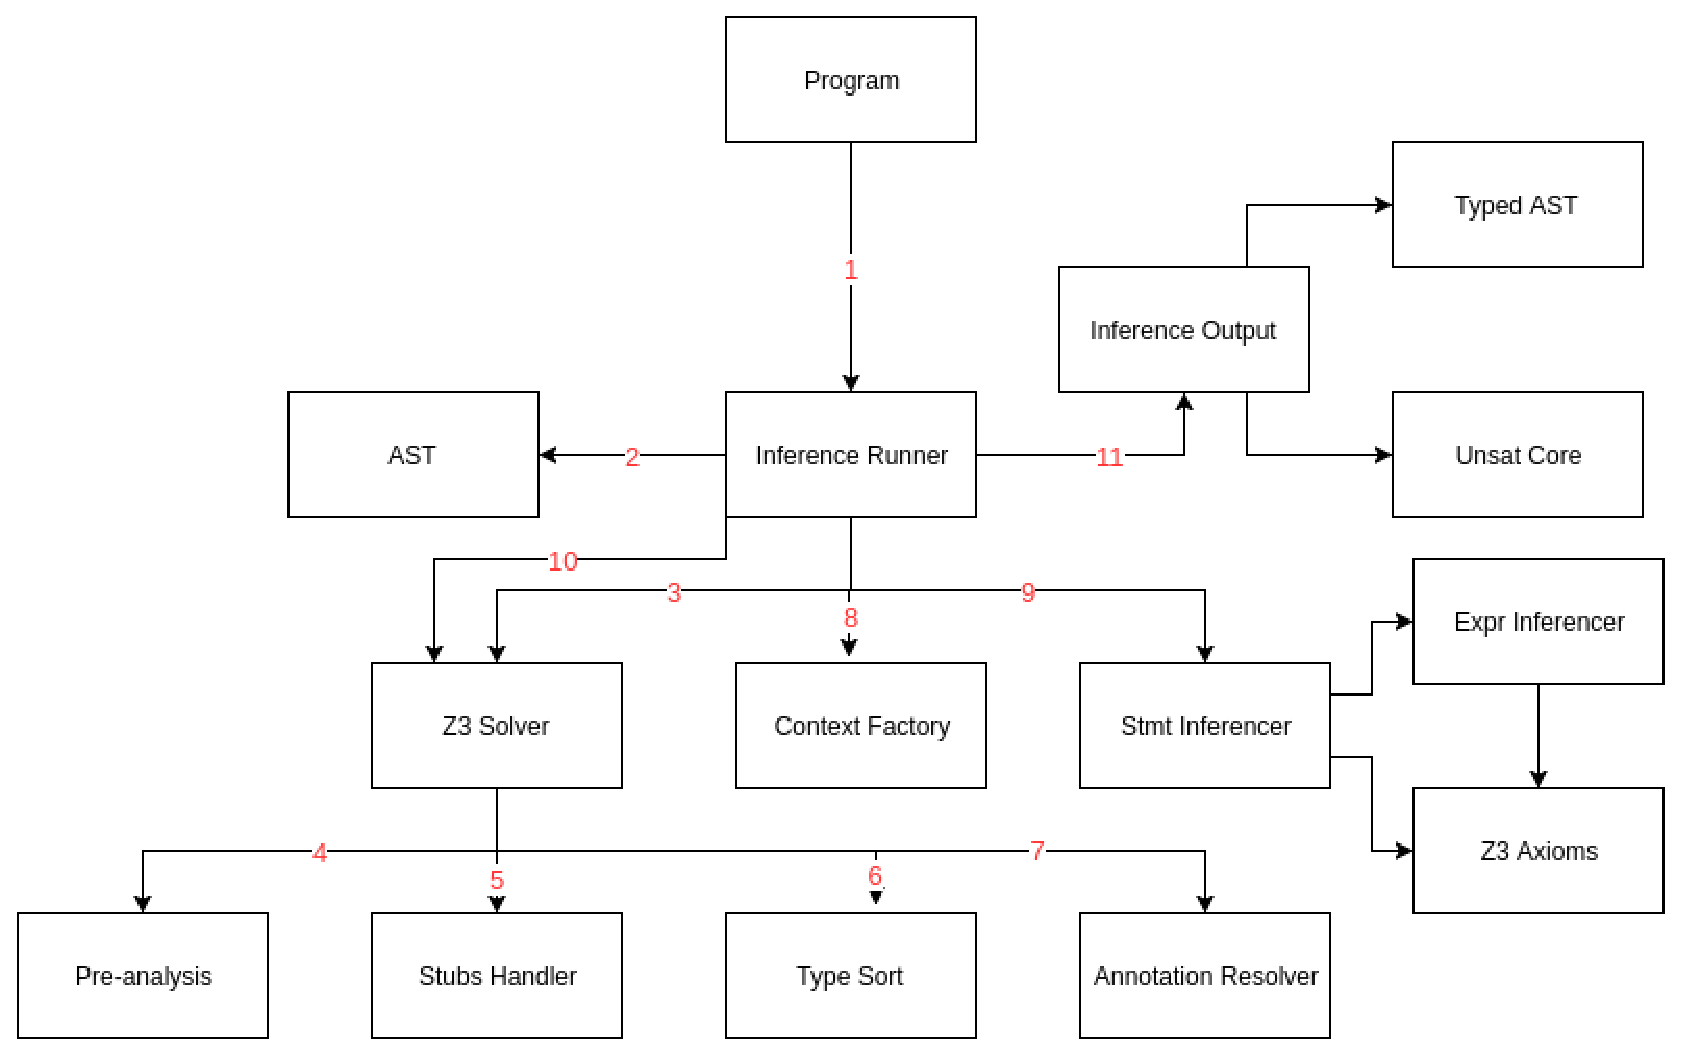
\includegraphics[width=130mm]{images/TI_comp.eps}\\
	\end{mdframed}
	\caption{Components of the Type Inference}
	\label{fig:ti_comp}
\end{figure}

Having explained the static type system in Chapter \ref{chapter:ts} and the design and the rules of the type inference in this chapter, we present in the next chapter the experimentation we performed to evaluate the type inference, and we discuss the limitations of the type inference and the cases it cannot handle.